\documentclass[journal]{IEEEtran}

\usepackage{graphicx} 
\usepackage{caption} 
\usepackage{siunitx} 
\usepackage{subcaption} 
\captionsetup[table]{skip=10pt}
\usepackage[margin=1in]{geometry} 
\usepackage{amsmath,amsthm,amssymb}
\usepackage[noend]{algpseudocode}
\usepackage{float}
\makeatletter
\def\BState{\State\hskip-\ALG@thistlm}
\makeatother

\graphicspath{{media/}}

\begin{document}

\title{Team 9 ROB 550 BotLab}

\author{Peter Mitrano, Sid Dey, Nathaniel Cox}

\maketitle

\begin{abstract}
In the BalanceBot lab, teams are tasked with
\end{abstract}
\IEEEpeerreviewmaketitle

\section{Introduction}
\IEEEPARstart{T}{h}e goal of the BotLab is to \dots

In this report, we discuss our implementation of SLAM, report on our systems accuracy and performance, and discuss our approach to several specific challenges like frontier exploration and the ``kidnapping'' problem.

\section{Methods}

Our SLAM algorithms consists of iteratively performing a localization step then a mapping step. On top of this, we plan paths through using A* on our occupancy grid and follow these paths with a proportional controller.
\subsection{Monte Carlo Localization}

\subsubsection{Occupancy Grid}

Include an image of your map from the log file obstacle\_slam\_10mx10m\_5cm.log

\begin{figure}[b]
    \centering
    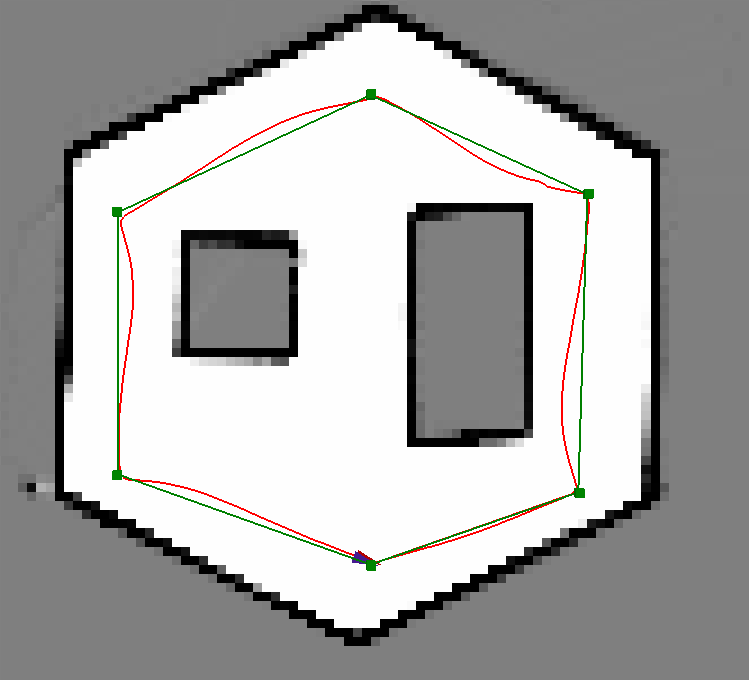
\includegraphics[width=1\linewidth]{obstacle_slam_10mx10m_5cm-map.png}
    \caption{Map built on the log file obstacle\_slam\_10mx10m\_5cm.log. True pose of the robot is shown in red.}
    \label{fig:map}
\end{figure}


\subsubsection{Action Model}

Describe the action model you used.  Include the equations you used
Include a table of the values of any uncertainty parameters.  
Explain how you chose these values.
 \subsubsection{Sensor Model}

Describe the sensor model you implemented.

\subsubsection{Particle Filter}

\begin{table}[b]
    \centering
    \begin{tabular}{|c|c|} \hline
         \# Particles & Time (ms) \\
         100 & 28 \\ \hline
         200 & 48 \\ \hline
         300 & 68 \\ \hline
         500 & 126 \\ \hline
         1000 & 250 \\ \hline
    \end{tabular}
    \caption{Time to update the particle filter. Each time was computed as the average of 10 updates.}
    \label{tab:filter_perf}
\end{table}

we fit a line to the data and calculated that we could handle $\approx400$ particles at \SI{10}{\hertz}.

\begin{figure}[b]
    \centering
    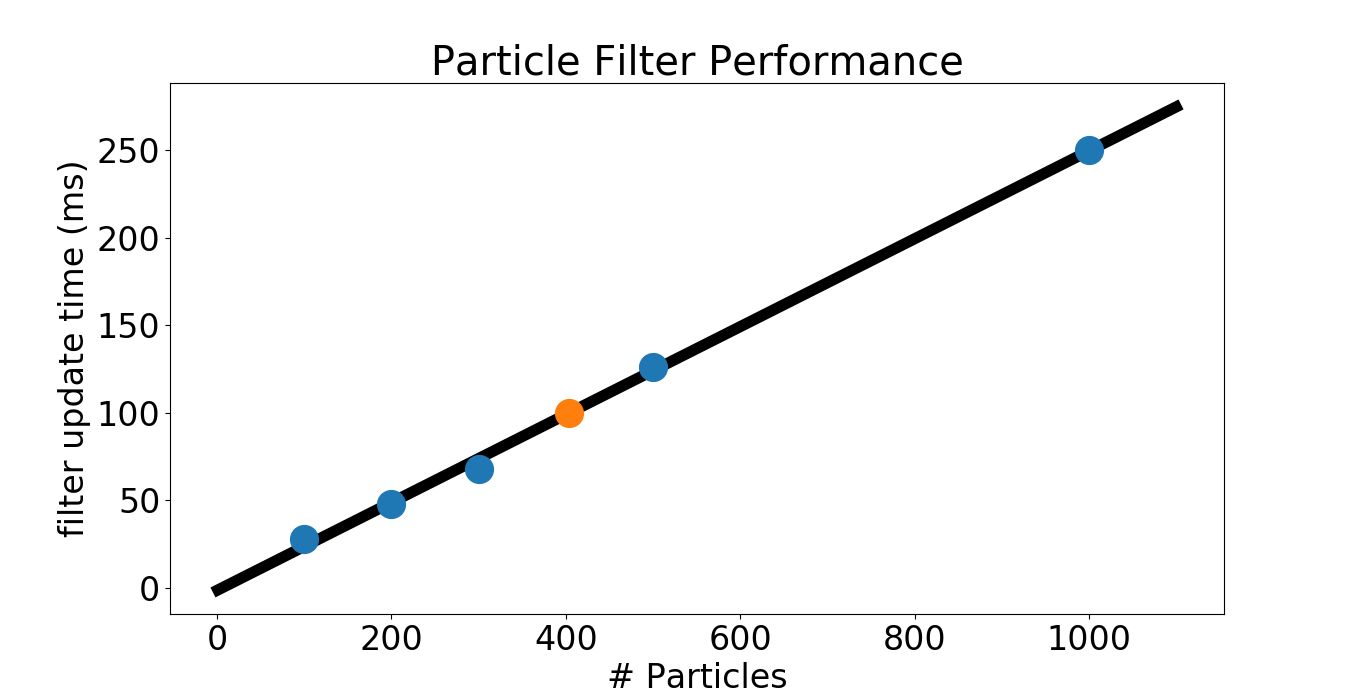
\includegraphics[width=1\linewidth]{filter_perf.png}
    \caption{Performance of the particle filter.}
    \label{fig:perf}
\end{figure}

\begin{figure}[b]
    \centering
    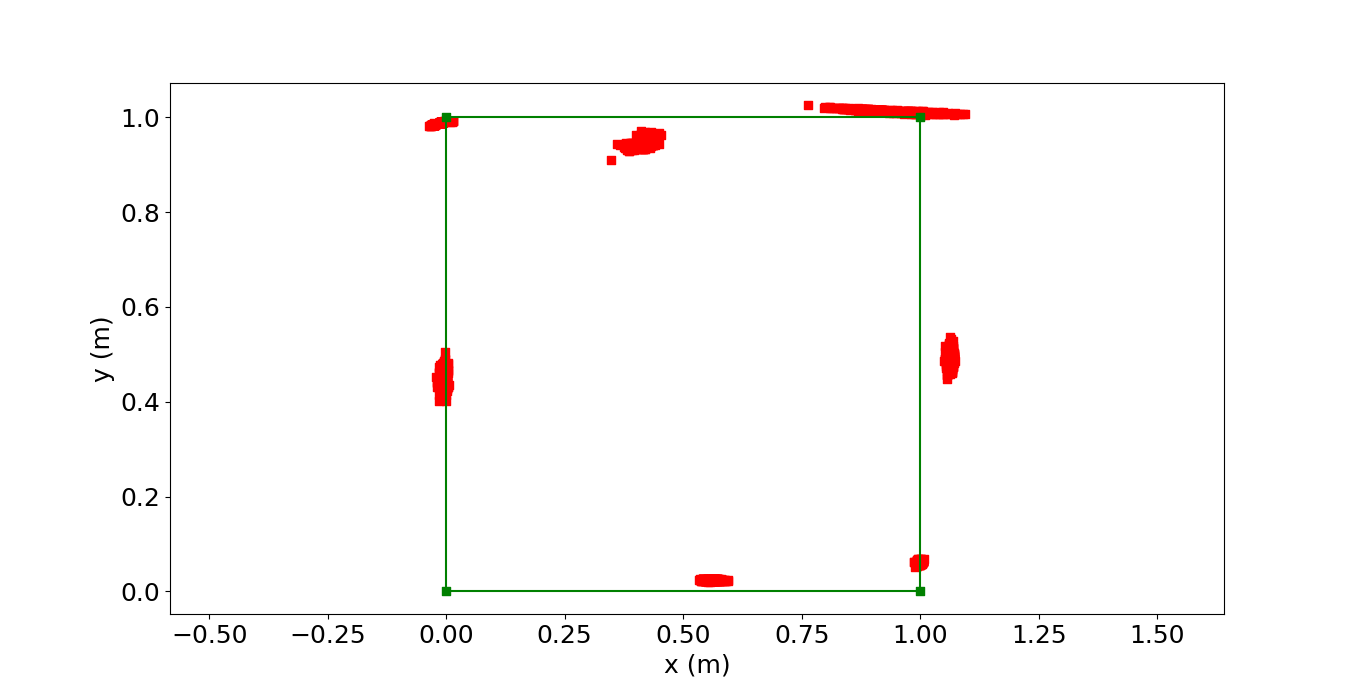
\includegraphics[width=1\linewidth]{drive_square_particles.png}
    \caption{Particles shown at various positions along a square path. Note that uncertainty is higher along the direction of motion.}
    \label{fig:square_particles}
\end{figure}

\subsection{SLAM}

Create a block diagram of how the SLAM system components interact

\begin{figure}
    \centering
    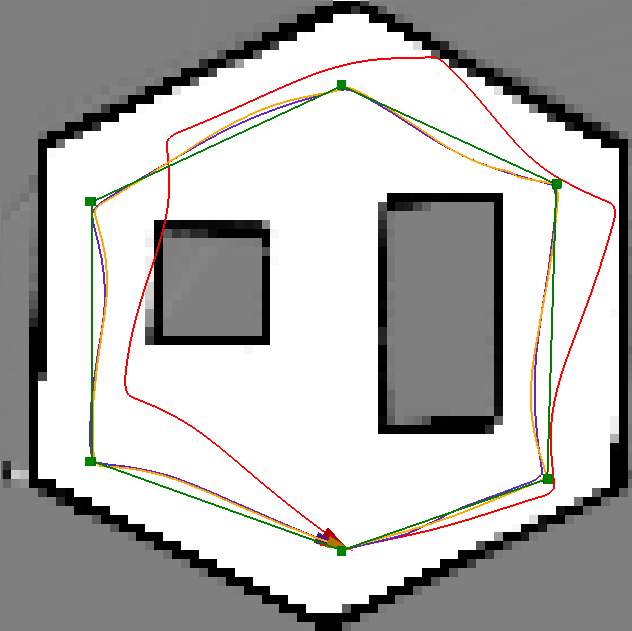
\includegraphics[width=1\linewidth]{obstacle_slam_10mx10m_5cm.png}
    \caption{Testing Localization only on obstacle\_slam\_10mx10m\_5cm.log.}
    \label{fig:localization}
\end{figure}

\begin{table}[b]
    \centering
    \begin{tabular}{|c|c|c|c|} \hline
      & Mean (m) &   Std dev &   Max (m) \\ \hline
      Odometry & 0.208  & 0.186  &  0.542 \\ \hline
      SLAM & 0.039 & 0.039 &  0.217 \\ \hline
    \end{tabular}
\caption{Statistics of the pose error for obstacle\_slam\_10mx10m\_5cm.log}
    \label{tab:localization_error}
\end{table}

\begin{figure}[t]
    \centering
    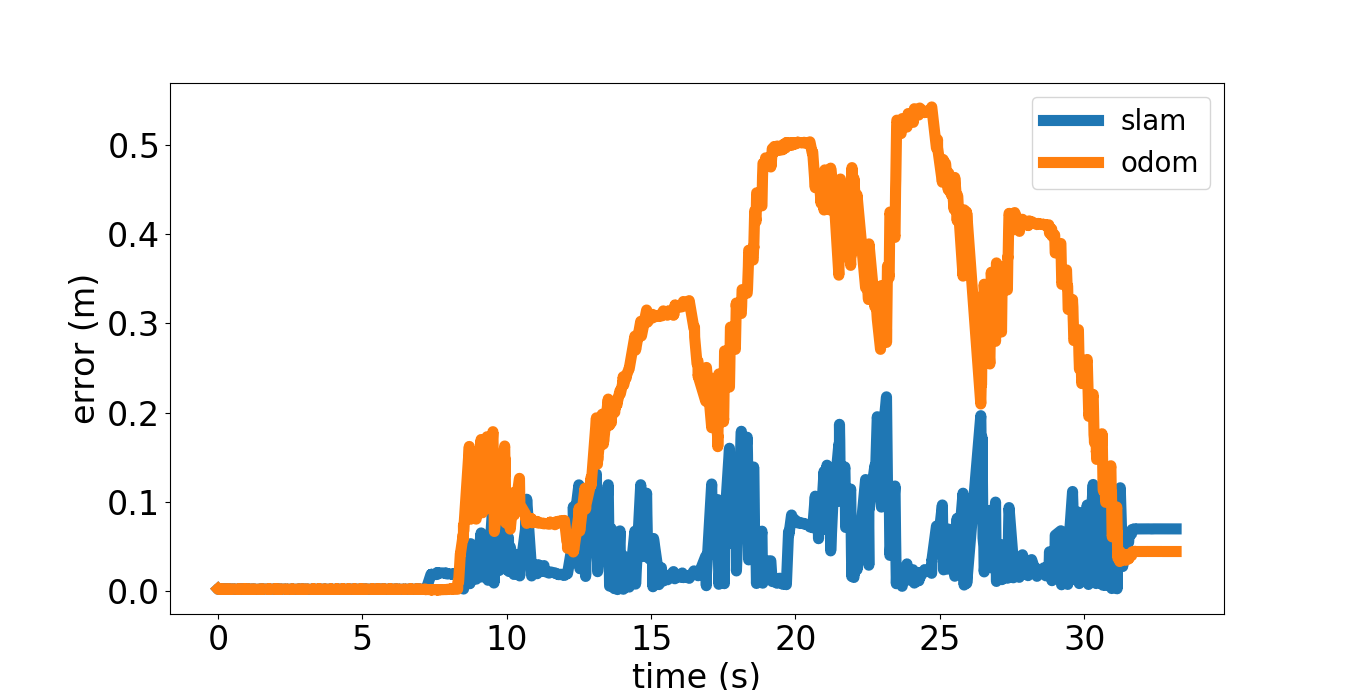
\includegraphics[width=1\linewidth]{localization_error.png}
    \caption{Error over time with respect to motion capture on the obstacle\_slam\_10mx10m\_5cm.log.}
    \label{fig:localization_error}
\end{figure}


\begin{figure}[t]
    \centering
    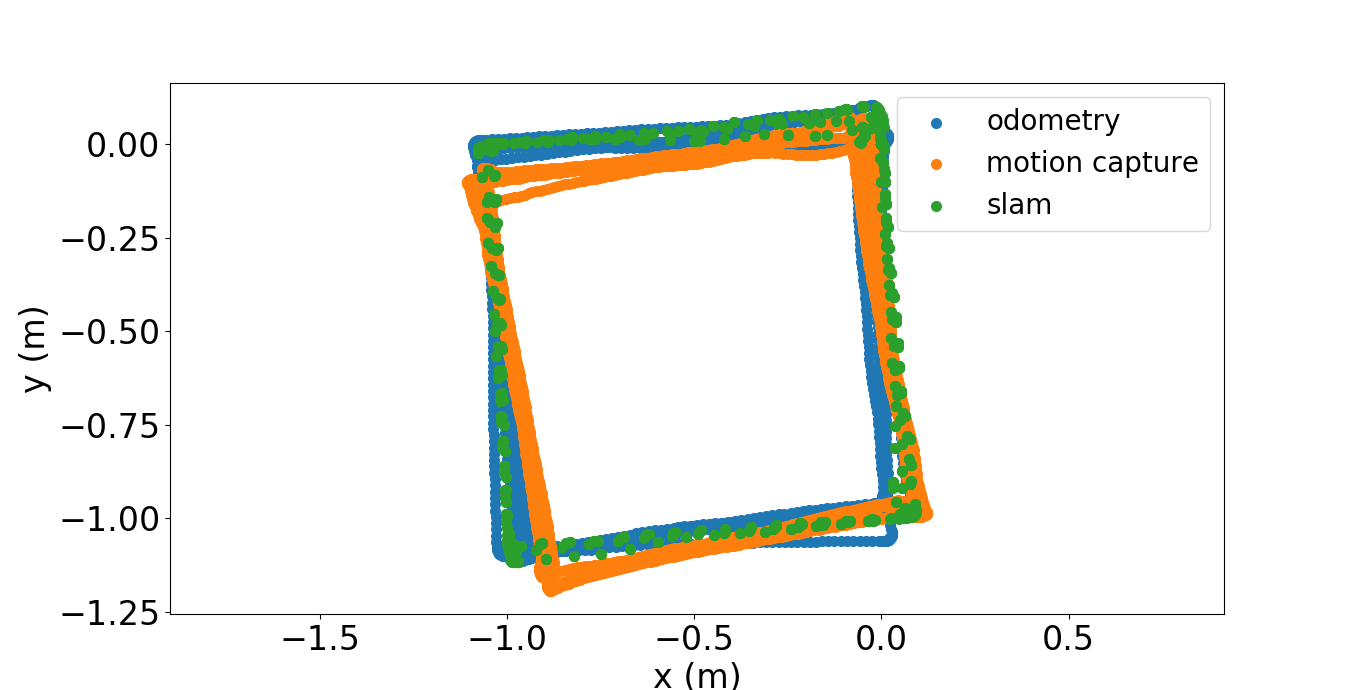
\includegraphics[width=1\linewidth]{slam_squares.png}
    \caption{SLAM Pose estimate versus motion capture pose.}
    \label{fig:slam_squares}
\end{figure}

\begin{figure}
    \centering
    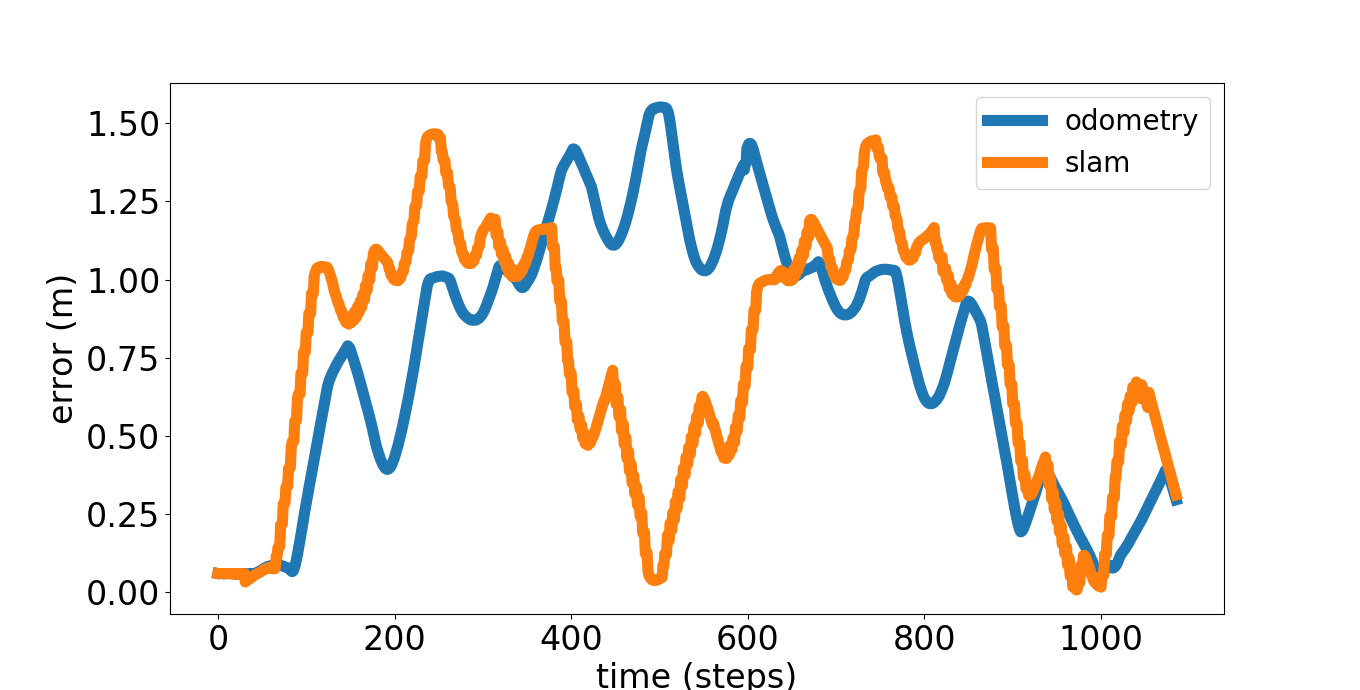
\includegraphics[width=1\linewidth]{slam_squares_error.png}
    \caption{Error over time with respect to motion capture.}
    \label{fig:slam_squares_error.}
\end{figure}

\subsection{Exploration}

Exploring the environment to build a complete map was one of the tasks. After we build our initial map and have localized, we chose a cell near the frontier and use A* to plan a path to that cell. By iteratively choosing cells near the frontier to visit, we eventually build up a complete map of the environment.

Our method for choosing which cell to explore starts with selecting the frontier whose centroid is furthest from the robots current position to explore. Next, we iterate over each cell in the frontier until we find one which is safe to navigate to. If we cannot do this, then we will continue on to search through cells in the next frontier.

We discuss the successes and failures of this method in the results and discussion sections.

\subsubsection{A* Path Planning}

Our A star algorithm was able to correctly find the optimal path in all of the provided test environments. Furthermore, the mean planning time on the realistic maze scenario was \SI{2.625}{\milli\second}, which is faster then the update period of our SLAM algorithm ($\approx$\SI{100}{\milli\second}). Therefore, our planner is fast enough to operate every cycle if necessary.

\begin{table}
    \centering
    \begin{tabular}{|c|c|c|c|c|c|} \hline
        & \multicolumn{5}{c|}{Planning Time (us)} \\ \hline
        Environment & min & mean & max & median & stdev \\ \hline
        convex & 194 & 197 & 218 & 195 & 7 \\ \hline
        empty & 5332 & 5630 & 6171 & 5468 & 295 \\ \hline
        maze & 2084 & 2625 & 3217 & 2533 & 410 \\ \hline
        narrow & 5404 & 136776 & 271503 & 69468 & 131305 \\ \hline
        wide & 5420 & 93529 & 268662 & 11361 & 122841 \\ \hline
    \end{tabular}
    \caption{A* Planning Times on the provided example problems. Statistics are computed on 20 trials on each map.}
    \label{tab:a_star_times}
\end{table}


\subsection{Motion Controller}

Given our localized position and a series of waypoints we intend to follow, we use one of two proportional controllers to navigate along these waypoints. First, we turn to face the current target waypoint, then we follow the straight line towards that waypoint. Our controller outputs a variable forward $v$ and rotational velocity $\omega$, much like the Dubins car model. In the turning face, these control velocities are computed according to the proportional control laws \eqref{eq:turn}. We then clip the rotation velocity such that $-1 < \omega < -0.1$ or $0.1 < \omega < 1$. Here we denote the angle from the robots current pose to the target waypoint as $\phi$ and the robots current heading $\theta$. The function $d$ gives the signed smallest angle in radians between two vectors in the range $[-\pi,\pi]$. We exit the turning mode when our $d(\phi,\theta) < 0.1$.

\begin{equation} \label{eq:turn}
    \begin{split}
     v &= 0 \\
     \omega &= \text{clamp}\Big[K_\text{turn}d(\phi,\theta)\Big]
    \end{split}
\end{equation}

After turning, we switch our control laws and drive towards the target waypoint. Once again, there are two cases to consider. In the case that the current waypoint is not the final waypoint in our overall plan, we move with a constant velocity of \SI{0.1}{\meter\per\second}. Otherwise, we use Equation \eqref{eq:fwd} to compute our control. The speed is clamped such that $-0.1 < v < -0.05$ or $0.05 < v < 0.1$. We discuss the decision to move at constant speed for all intermediate waypoints in the Discussion section.

\begin{equation} \label{eq:fwd}
    \begin{split}
     v &=  \text{clamp}\Big[K_\text{fwd}||p, g||_2\Big] \\
     \omega &= \text{clamp}\Big[K_\text{turn2}\big(||p, g||_2+0.01\big)d(\phi,\theta)\Big]
    \end{split}
\end{equation}

The desired forward and rotational velocities and then converted to wheel speeds using Equation \eqref{eq:wheel_speeds}. Here $v_l$ is the left wheel speed in \SI{}{\radian\per\second} and $v_r$ is the right wheel speed, and $W$ is the distance between the wheels. The turning speeds and wheel speeds are controlled by a PID controller within the provided Mobilebot program. Additionally, the Mobilebot program uses a low pass filter to mitigate potential noise in velocity estimates. PID constants and filter parameters used are shown in Table \ref{tab:pid}.

\begin{equation} \label{eq:wheel_speeds}
    \begin{split}
        v_l &= v - \omega\frac{W}{2} \\
        r_l &= v + \omega\frac{W}{2}
    \end{split}
\end{equation}

\begin{table}[b!]
    \centering
    \begin{tabular}{|c|c|c|c|} \hline
        kP & kI & kD & Filter Hz \\ \hline
        1.0 & 0.0 & 0.0 & 25 \\ \hline
        1.0 & 0.0 & 0.0 & 25 \\ \hline
        0.05 & 0.0 & 0.0 & 10 \\ \hline
        0.05 & 0.0 & 0.0 & 10 \\ \hline
    \end{tabular}
    \caption{PID constants used in the provided Mobilebot program}
    \label{tab:pid}
\end{table}

Include a plot of your robot’s dead reckoning estimated pose and the ground truth pose from the optitrack system as the robot is commanded to drive a square 4 times using the drive\_square program.

\begin{figure}[b]
    \centering
    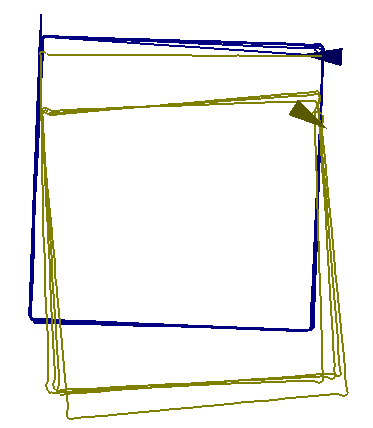
\includegraphics[width=1\linewidth]{odometry4.png}
    \caption{Plot of our robot performing four \SI{1}{\meter} squares. Blue is pose estimate from odometry, yellow is the motion capture pose.}
    \label{fig:odometry_squares}
\end{figure}

\section{Results}

\section{Discussion}

\subsection{Motion Controller}

When we first used our motion controller to follow paths, we noticed that the robot spent a lot of time turning to follow waypoints that are space very close together. This meant that the robot took a long time to follow a path. To mitigate this, we both increased the position and angle tolerance for intermediate waypoints and also chose to fix the forward speed when navigating to intermediate waypoints. This way the robot did not stop, in the event that the next waypoint is in a straight line, which was often the case in our experience, that path is execute more smoothly and more quickly.

\section{Conclusion}

Group 9 successfully completed the BotLab lab, ...

\bibliographystyle{IEEEtran}
\bibliography{550-botlab}

\newpage

\section{Appendix}

\end{document}